\section{Introduction}
\label{sec:intro}

\sam{}~\cite{carion2026sam3} turns promptable segmentation into concept segmentation: given a short noun phrase, an image exemplar, or both, it returns a mask for every instance of the concept.
A model with an open vocabulary is asked, most of the time, about things that are not in the image, so its ability to return nothing matters as much as the quality of its masks.
\sam{} assigns that ability to one component.
A learned presence token predicts whether the concept is in the image, and the score of every proposal is multiplied by that prediction.
The authors credit this presence head, together with hard negative phrases in the training data, for the model's image-level recognition~\cite{carion2026sam3}.

\sam{} also accepts image exemplars: boxes labelled positive or negative, alone or next to a phrase.
Exemplars are how the model is put to work beyond text prompting.
Few-shot segmentation places a support image beside the query and passes the support box as a positive exemplar~\cite{tsai2026fss,tsai2026case}.
Exemplar-based counting passes a box around one instance~\cite{ranjan2021fsc,amini2024countgd}.
Detect-then-segment pipelines in the style of Grounded SAM pass a detector's boxes~\cite{ren2024groundedsam}.
An annotator adds a box where the model missed an object~\cite{carion2026sam3}.
In each case a box is supplied before anyone knows whether the named concept is in the image, and the presence head is the only part of the model that could say that it is not.

This paper shows that it does not.
With a positive exemplar in the prompt, the presence head stops rejecting.
On 500 held-out LVIS~\cite{gupta2019lvis} images, for categories that the annotators verified to be absent, the presence logit is non-negative in 1.6\% of text-only prompts and in 99.5\% of prompts that add one positive box (\cref{tab:veto}).
The model then returns the boxed object as an instance of the absent concept in 96.8\% of cases, with the presence logit at its upper clamp in 59\%.
\Cref{fig:qualitative} shows two cases: a pair of jeans returned as a ``coconut'' and a giraffe returned as a ``wine bucket''.

What the box contains does not matter.
A box placed on the least-annotated region of the image keeps the presence logit non-negative in 99.6\% of cases.
So do boxes at half scale, at double scale, and shifted by half their width, and so do two or three boxes.
A lone \emph{negative} box does the opposite and pins the logit at its lower clamp (\cref{tab:controls}).
The head behaves as if it read the exemplar's label and not the image.
That is what the published training protocol would teach it: positive exemplars are sampled from the ground-truth boxes of missed instances, so a positive box always accompanies a concept that is present, and exemplar prompting was evaluated only on images that contain the concept~\cite{carion2026sam3}.
We offer this as an account that agrees with the protocol and with our controls.
We did not retrain the model to test it.

The image features are shared across prompts, so the text-only presence costs one more decoder pass.
We gate the exemplar pass on it and discard its output when the text-only presence probability is below 0.10.
On the held-out images the gate cuts absent-phrase episodes that return a mask from 99.5\% to 6.4\% and costs 0.002 mIoU when phrase and box agree (\cref{tab:gates}).
On FSC-147~\cite{ranjan2021fsc} it cuts false counts for an absent class from 85.5\% to 4.3\%.
As a verifier of detector boxes, \sam{} without the gate accepts 99.7--100\% of boxes whose class is not in the image.
With the text-only presence in its score it separates correct from class-absent boxes with an AUROC of 0.96, above the confidence of both detectors we tried (\cref{tab:detector}).

Every threshold in this paper was fixed before the run it scores.
Of 27 such criteria, 23 passed.
The four that failed include the first version of our gate and a geometric variant of it, and we report them with the rest (\cref{tab:criteria}).
Our contributions are:
\begin{itemize}[leftmargin=*,itemsep=1pt,topsep=2pt]
    \item A measurement, on three image sets and 4,500 absent-phrase episodes, that a positive exemplar removes \sam{}'s rejection of absent concepts.
    \item Controls that separate the exemplar's label from its content, with a negative-exemplar prediction that holds.
    \item A training-free gate, selected on one image set and confirmed on a disjoint one under criteria fixed in advance, with two alternatives that failed.
    \item The consequences for two uses of exemplars, detector verification and counting, including what the gate does not fix.
\end{itemize}

\begin{figure*}[t]
    \centering
    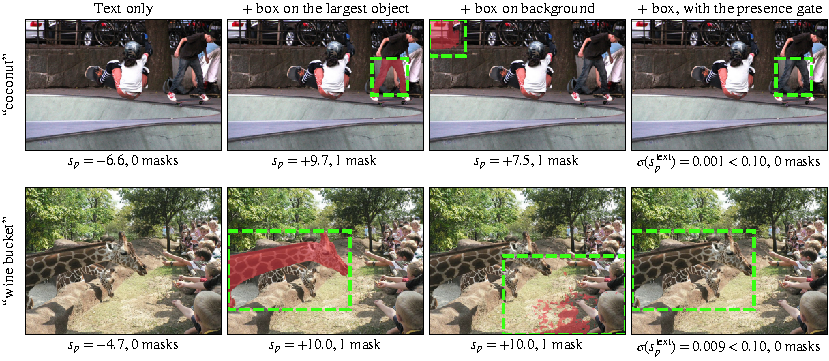
\includegraphics[width=\linewidth]{fig/qualitative.pdf}
    \caption{\textbf{A positive box makes \sam{} accept an absent concept.}
    Each row is one image and one phrase for a category that LVIS verifies to be absent.
    Text alone is rejected: the presence logit $\spres$ is negative and no mask is returned.
    Adding a positive exemplar box (dashed) drives $\spres$ to its upper range, and the boxed object is returned as the concept.
    A box on the least-annotated region has the same effect.
    Gating on the text-only presence probability restores the rejection.
    The images are the first two held-out images by id that are landscape and whose largest object covers 5--40\% of the frame; they were not chosen by outcome.}
    \label{fig:qualitative}
\end{figure*}
